\documentclass[11pt]{article}
\usepackage{graphicx} % Required for inserting images
\setlength{\parindent}{0pt}
\usepackage[bookmarks=true, colorlinks=true, urlcolor=blue, linkcolor=black]{hyperref}

\usepackage{enumitem}
\usepackage[utf8]{inputenc}
\usepackage[T1]{fontenc}
\usepackage[english]{babel}
\usepackage{geometry}
\usepackage{lastpage}
\usepackage{fancyhdr}
\usepackage{datetime}

% % Link to other SOPs, forms
% \usepackage{xr}
% \externaldocument[102-]{../2_medical/sop_102_medical}

% figures and tables
\usepackage{graphicx}
\graphicspath{ {../../pics} }
\usepackage{rotating}
\usepackage{float}
\usepackage{subfig}
\usepackage{caption}
\DeclareCaptionLabelFormat{adja-page}{\hrulefill\\#1 #2 \emph{(previous page)}}


\renewcommand{\headrulewidth}{0pt}
% \newdateformat{yearmonth}{\THEYEAR-\THEMONTH-\THEDAY}
\pagestyle{fancy}
\fancyhead[L]{}
\fancyhead[R]{Approved: TBD}
\fancyfoot[C]{}
\fancyfoot[L]{ND-HNC SOP 301: v.0.1.0}
\fancyfoot[R]{p. \thepage /\pageref*{LastPage}}


% start document
\begin{document}

\renewcommand{\labelenumii}{\arabic{enumi}.\arabic{enumii}}
\renewcommand{\labelenumiii}{\arabic{enumi}.\arabic{enumii}.\arabic{enumiii}}
\renewcommand{\labelenumiv}{\arabic{enumi}.\arabic{enumii}.\arabic{enumiii}.\arabic{enumiv}}

\begin{center}
	\textbf{\Large SOP 301: Building Access}\\
	\hrulefill
\end{center}


\section{Summary}
This document establishes procedures for building access of the Notre Dame Human Neuroimaging Center (ND-HNC), located in the Lower Level of:\\

Veldman Family Psychology Clinic\\
501 North Hill St.\\
South Bend, IN 46617

\section{Scope}
These policies apply to all investigators, research assistants, and staff who use the ND-HNC.

\section{Definitions}

TBD
% \begin{itemize}
% 	\item \textbf{Experimenter}: The investigator, research assistant, or MRI operator who is responsible for the subject and conducting the experiment.
% 	\item \textbf{Electronic Lock}: All external doors to the Veldman Family Psychology Clinic (VFPC), the ND-HNC, and the ND-HNC MRI Zones are controlled by electronic locks. A single electronic key card is used for entry. The electronic lock system recognizes the owner's Irish1Card (ND ID/phone), logs the time of the attempted entry, and unlocks the door if the owner has been granted access.
% \end{itemize}


\section{Notes}

None


\section{Policies \& Procedures}

Procedures to access the building during and outside normal business hours, hosting visitors, and key/card access are detailed. For specific policies and procedures related to access of MRI and various MRI zones, please refer to [TODO SOP].

% Enter normal
\subsection{Entering Building: Normal Business Hours}
\label{ssec:enter-norm}

Normal building business hours Monday through Thursday are 7am-7pm. Friday hours are 7am-4pm. The exterior door to the main entrance is unlocked during normal hours [TODO PIC?].

\begin{enumerate}
	\item \textbf{Enter via main entrance}: go through the interior main entrance door either by being let in by someone at the Veldman Center reception desk, or by using your Irish1Card and PIN (Fig. \ref{fig:vfpc-card}).
	\item \textbf{Enter via staff entrance}: use your Irish1Card and PIN.
	\item Sign in at the first floor reception logbook.
	\item Proceed to your destination which may require the use of:
	\begin{enumerate}
        \item Your Irish1Card (for doors in non-public areas on each floor),
        \item Physical key (for private offices),
        \item Code (for shared spaces).
    \end{enumerate}
\end{enumerate}


% Enter outside normal
\subsection{Entering Building: Outside of Normal Business Hours}
\label{ssec:enter-outnorm}

Outside of normal business hours you will need the following to access the building:

\begin{enumerate}
	\item Irish1Card,
	\item A personal PIN (4-digit code associated with the Irish1Card),
	\item An alarm code (6-digit code arranged with security),
	\begin{enumerate}
        \item This can be arranged through an ND-HNC staff member.
    \end{enumerate}
\end{enumerate}

To enter:
\begin{enumerate}
    \item Present your Irish1Card by holding it close to the keypad (light should flash green).
    \item Enter the PIN associated with Irish1Card.
    \item Open the door once it unlocks.
    \item Disable building alarm:
    \begin{enumerate}
        \item Enter your 6-digit code by touching the numbers on the keypad (Fig. \ref{fig:vfpc-alarm}).
        \item Hit the 'Enter' button to the top-right on the keypad.
    \end{enumerate}
    \item Sign in at the first floor reception logbook.
\end{enumerate}


% Host visitors
\subsection{Hosting Visitors}
\label{ssec:host-visit}

All visitors will be greeted in the first floor reception area using the main entrance. Visitors mut be greeted in reception and then escorted to ND-HNC.

\begin{enumerate}
	\item Visitors can be let in by:
	\begin{enumerate}
        \item Physically opening the door
        \item Using the wheelchair access buttons (not recommended for sensory sensitive visitors as it is very loud)
        \item Using the remote release button at the reception desk
        \item Using the phone/intercom system
    \end{enumerate}
    \item Do not have them sign in at the front desk in order to maintain their anonymity and confidentiality
    \item Visitors must be escorted and monitored at all times
    \item Escort them back to the first floor reception area at the end of their visit.
\end{enumerate}


% Exit building normal
\subsection{Exit Building: Normal Business Hours}
\label{ssec:exit-norm}

\begin{enumerate}
	\item Sign out of logbook at first floor reception.
\end{enumerate}


% Exit building out normal
\subsection{Exit Building: Outside Normal Business Hours}
\label{ssec:exit-outnorm}

\begin{enumerate}
	\item Sign out of logbook at first floor reception.
	\item Using the logbook, confirm whether anyone remains in the building.
	\item If last, activate building security:
	\begin{enumerate}
        \item Verify the green checkmark appears on the keypad.
        \item Enter your 6-digit alarm code.
        \item Press 'Enter'.
    \end{enumerate}
\end{enumerate}


% Key access
\subsection{Key Access}
\label{ssec:keys}

\begin{enumerate}
	\item Master keys: available only at lockbox.
	\item Room keys: contact ND-HNC staff.
\end{enumerate}


% Card access
\subsection{Card Access}
\label{ssec:card}

\begin{enumerate}
	\item Irish1Card required for building, MRI Zone access.
	\item Set, access PIN: \url{https://idcardpin.nd.edu}
\end{enumerate}


\section{Figures}

% Card access
\begin{figure}[H]
	\centering
	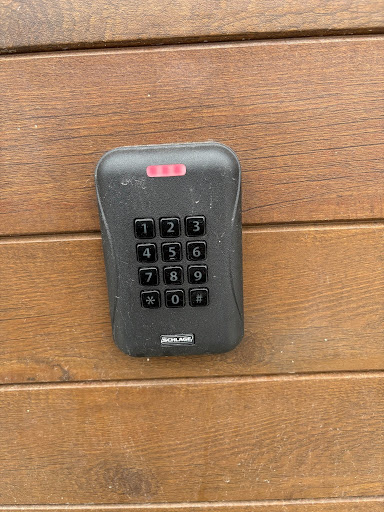
\includegraphics[width=0.8\textwidth]{vfpc_card_access.jpg}
	\caption{VFPC exterior door keypads}
	\label{fig:vfpc-card}
\end{figure}

% Alarm panel
\begin{figure}[H]
	\centering
	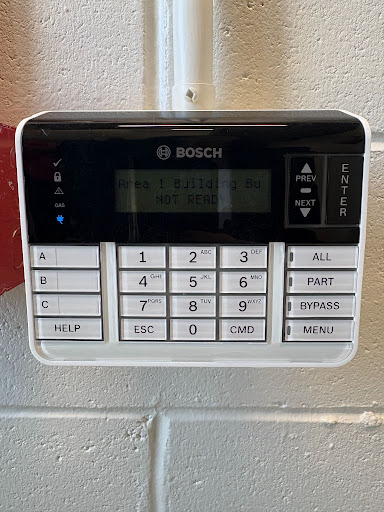
\includegraphics[width=0.8\textwidth]{vfpc_alarm.jpg}
	\caption{VFPC exterior door keypads}
	\label{fig:vfpc-alarm}
\end{figure}


\end{document}